\documentclass{elsarticle}
%\usepackage[pdftex,breaklinks,linktocpage,pagebackref,hyperindex,hyperfigures]
\usepackage{hyperref}
\usepackage[utf8]{inputenc}
\usepackage{amsmath}
\usepackage{amsthm}
\usepackage{amssymb}
\usepackage[tmargin=1in,bmargin=1in]{geometry}
\usepackage{subfigure}
\usepackage{graphicx}
\usepackage{latexsym}
\usepackage{pdfsync}
\usepackage{caption}

\usepackage{algorithm}
\usepackage{algpseudocode}
\usepackage{multirow}
\usepackage{rotating}
\usepackage{color}
\usepackage{ulem}
\usepackage{wrapfig}
\usepackage{siunitx}

\journal{Journal of Computational Physics}

\hypersetup{
    colorlinks=true,      		% false: boxed links; true: colored links
    linkcolor=blue,       		% color of internal links
    citecolor=blue,       		% color of links to bibliography
    filecolor=black,      		% color of file links
    urlcolor=red,       		% color of external links
    %bookmarks=false,
    pdffitwindow=true,
    pdfpagelayout=SinglePage
}

\bibliographystyle{plain}



\newtheoremstyle{own}%
    {1pt}% Space above
    {1pt}% Space below
    {}% Body font
    {}% Indent amount
    {\color{black}\bfseries}% Theorem head font
    {:}% Punctuation after theorem head
    {1pt}% Space after theorem head
    {}% Theorem head spec
    
    
\theoremstyle{own}
\newtheorem{example}{Example}

\newtheorem*{remark}{Remark}

\algblock[parallel for]{ParFor}{EndParFor}


\newcommand{\giga}{\si{\giga}}
\newcommand{\second}{\si{\second}}
\newcommand{\kilo}{\si{\kilo}}
\newcommand{\meter}{\si{\meter}}
\newcommand{\comment}[1]{\textcolor{red}{#1}}
\newcommand{\milescomment}[1]{\textcolor{blue}{#1}}
\newcommand{\chohongcomment}[1]{\textcolor{green}{#1}}

\begin{document}


% declaration of the new block
\algblock{ParFor}{EndParFor}
% customising the new block
\algnewcommand\algorithmicparfor{\textbf{parallel\ for}}
\algnewcommand\algorithmicpardo{\textbf{do}}
\algnewcommand\algorithmicendparfor{\textbf{end\ parallel\ for}}
\algrenewtext{ParFor}[1]{\algorithmicparfor\ #1\ \algorithmicpardo}
\algrenewtext{EndParFor}{\algorithmicendparfor}


\title{Fast surface generation for biomolecular computations with the Voronoi Interface Method}	
%\author{Miles Detrixhe, Chohong Min, Fr\'ed\'eric Gibou}

\author{Miles Detrixhe}
\ead{mdetrixhe@engineering.ucsb.edu}
\address{Department of Mechanical Engineering \\
University of California Santa Barbara, Santa Barbara, CA, 93106}

\author{Mohammad Mirzadeh}
\ead{}
\address{MIT
}

\author{Arthur Guittet}
\ead{}
\address{
}

\author{Fr\'ed\'eric Gibou}
\ead{fgibou@engineering.ucsb.edu}
\address{Department of Mechanical Engineering \\
Department of Computer Science \\
Department of Mathematics \\
University of California Santa Barbara, Santa Barbara, CA, 93106}


\begin{abstract}
We improve upon the state-of-the-art level set surface generation technique for biomolecules by employing a fixed radius nearest neighbor search algorithm. By choosing an appropriate data structure we show that the time complexity of this algorithm is independent of the number of atoms in a particular biomolecule.
\end{abstract}

\begin{keyword}
  Parallel computing\sep 
  Poisson-Boltzmann equation \sep
  octree data structure \sep
  level set
\end{keyword}

\maketitle



\section{Introduction}


\section{Poisson-Boltzmann equations}

\section{Biomolecular surface description}

\section{fast surface generation}


The method of surface generation used in \cite{MirzadehTheillardHelgadottirEtAl:12:AdaptiveFiniteDifference} was a brute force implementation of a modified version of Nearest Neighbor Search. 

In the classic nearest neighbor search, given a query point, one aims to find the nearest element of a set of points. In computing the value of the level set function at a point, one aims to find the maximum value of the following function for all atoms in the molecule. 

\begin{equation*}
\phi(x,y,z) = \max_i\left\lbrace r_i - \sqrt{(x-x_i)^2 + (y-y_i)^2 + (z-z_i)^2} \right\rbrace
\end{equation*}

Because the reinitialization procedure is used to propagate the solution of $\phi$ away from the interface, it is sufficient to have an accurate method of computing $\phi$ near the interface. 

This reduces it to the fixed-radius nearest neighbor problem. This is an old problem (even for molecular applications \cite{Levinthal:66:Molecular-model-buil}) and there exist efficient ways of solving it e.g. \cite{Bentley:75:A-Survey-of-techniqu,Bentley;Stanat;Williams:77:The-complexity-of-fi}.

We use an octree data structure with each cell containing those atoms within a fixed radius of the center of the cell. The radius is related to the maximum atom radius plus the probe radius. 



For instance, consider the 3J6D protien from the PDB database. It has 131664 individual atoms. If we store those atoms in an octree such that each leaf cell contains all the atoms within a fixed radius from the cell center, then we get the figure below. This is for an atom tree with max level 7. The maximum number of atoms to be queried is 622. If no atoms are with the fixed radius of a leaf cell, then we populate that cell with the nearest atom.

\begin{figure}[ht]
\begin{center}
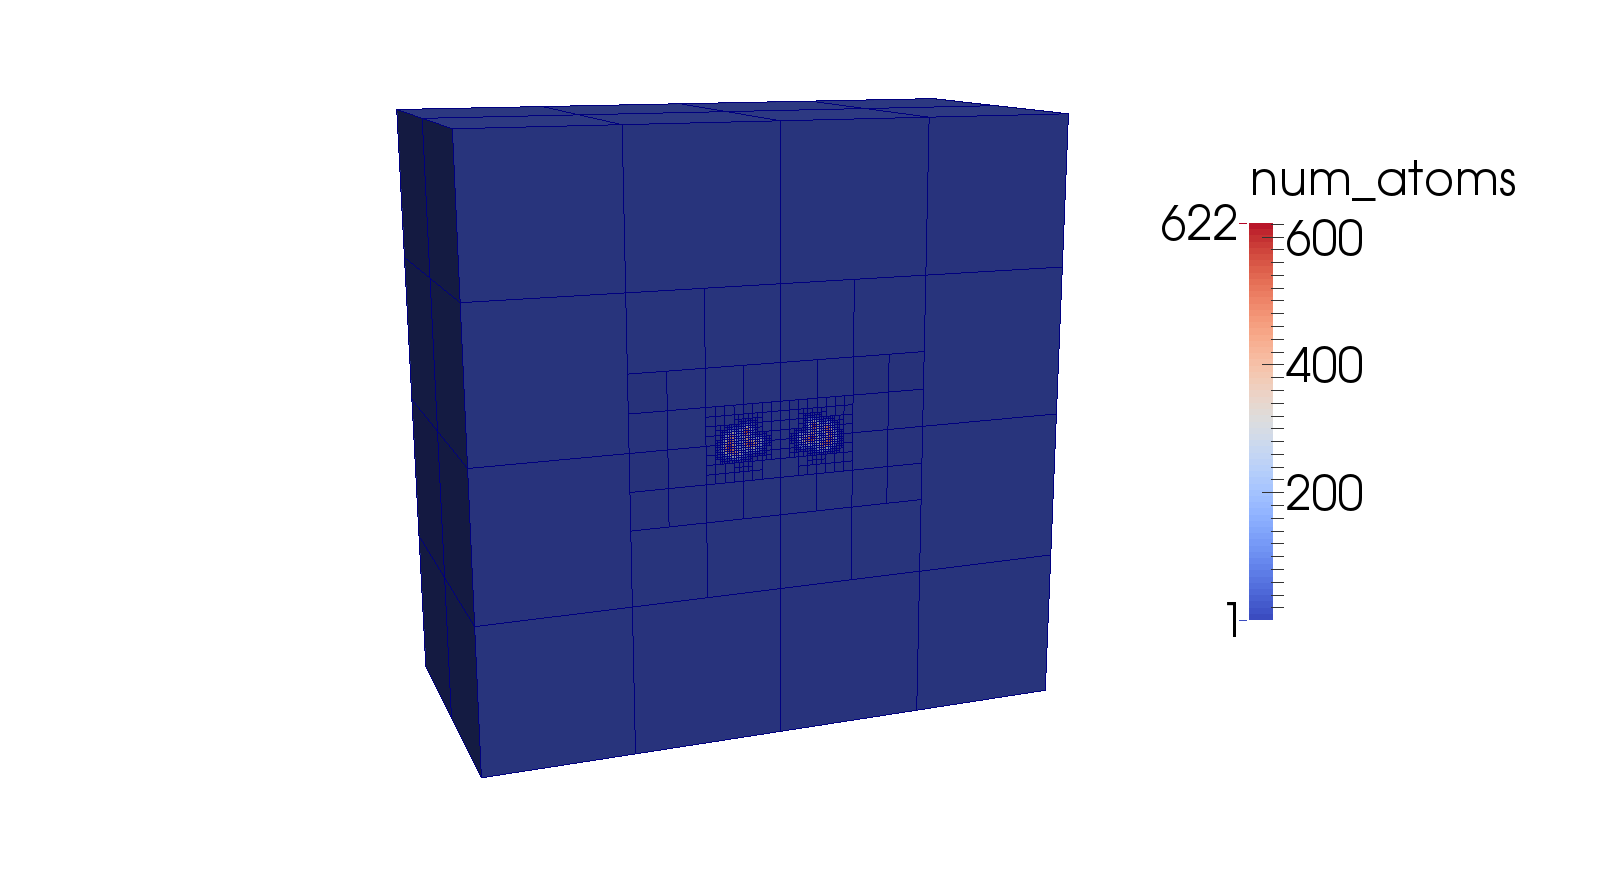
\includegraphics[width=0.945\textwidth]{../figs/atom_tree_3J6D}
\end{center}
\caption{Figure showing the atom tree data structure. It is a quadtree with max level 7. } \label{fig:atom_tree_3J6D}
\end{figure}



\section{solving PB on octree - Voronoi Interface method}

\section{Numerical examples}


\begin{figure}[ht]
\begin{center}
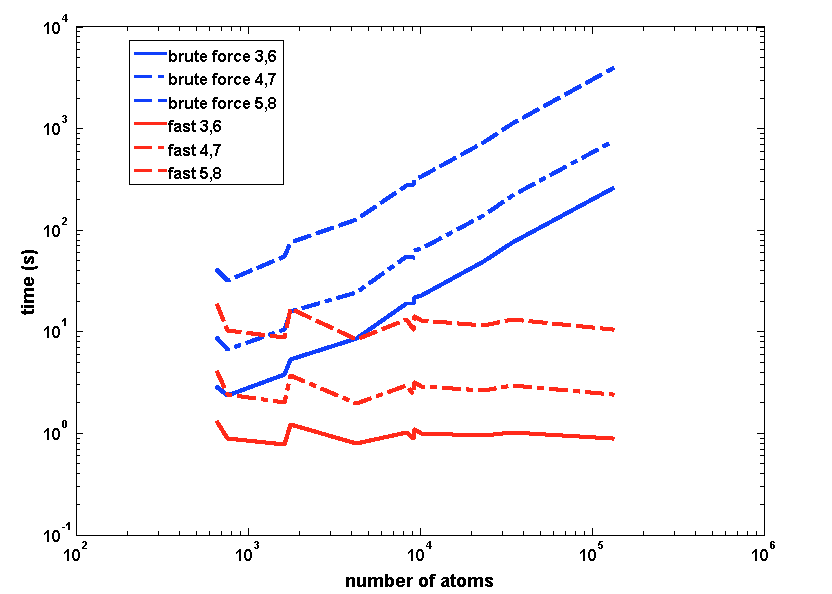
\includegraphics[width=0.945\textwidth]{../figs/fast_gen_timing}
\end{center}
\caption{Surface generated using 10 different molecules from the PDB database. Exact, brute-force method used as a benchmark.} \label{fig:fast_gen_timing}
\end{figure}


\begin{figure}[ht]
\begin{center}
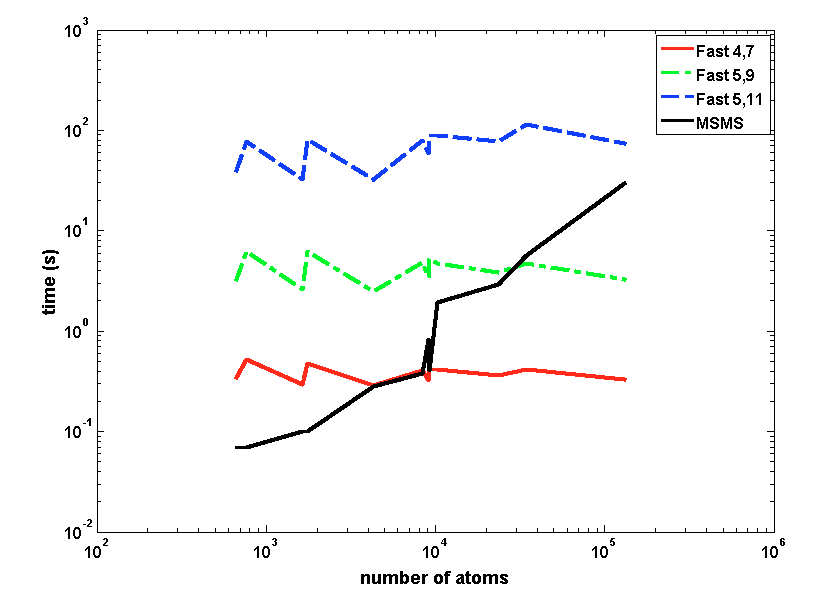
\includegraphics[width=0.945\textwidth]{../figs/timing_msms_compare}
\end{center}
\caption{Time to generate surface on various grid levels. MSMS timings used as a benchmark. This shows that for large atoms, this method is faster than MSMS even on relatively fine octrees (max level 11).} \label{fig:timing_msms_compare}
\end{figure}


\begin{figure}[ht]
\begin{center}
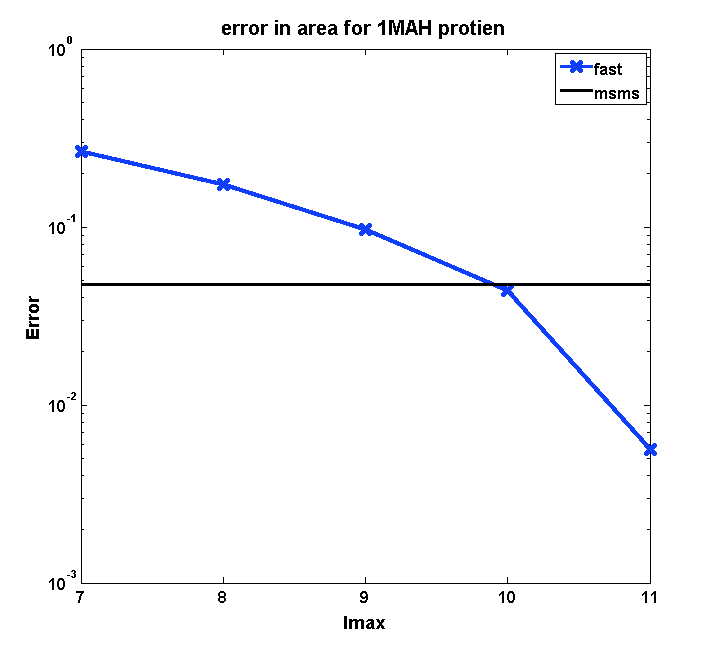
\includegraphics[width=0.945\textwidth]{../figs/error_convergence_1MAH}
\end{center}
\caption{Error in total computed surface area for the 1MAH protien level set method compared to MSMS. This shows that the surface area accuracy is competitive with MSMS for moderately refined grids (max level 10).} \label{fig:error_convergence_1MAH}
\end{figure}


\subsection{Fast surface generation}

MSMS \cite{Sanner;Olson;Spehner;etal:96:REDUCED-SURFACE:-an-}


%\begin{table}[h]
%\begin{center}
%   \begin{tabular}{| c |  c | c | c | c |}
%  \hline
%     PDB ID & \# Atoms & Analytical & Triangulated & Time msms \\ \hline
%	 1d65 &  760 & 3573.80 & 3405.72 & 0.07 \\ \hline
%	 6rxn & 1030 & 3827.86  & 4065.94  & 0.07 \\ \hline
%	 2err & 1638  & 4917.44  & 5189.28  & 0.10  \\ \hline
%	 1aa2 & 2145 & 5714.00 & 5389.36 & 0.10     \\ \hline
 %    2x6a & 4297  & 12969.68  & 13605.47  & 0.28  \\ \hline
%     3M3D &  8976 & 16626.72  & 17493.79   & 0.38  \\ \hline
%  	 1mah & 9133  & 19431.54  & 18509.91   & 0.83  \\ \hline
%	 1fss & 9360  & 19495.40  & 18581.67  & 0.41  \\ \hline
%     1OED & 10245   & 31013.07  & 32413.19  & 1.95 \\ \hline
%	 3ecd & 24749  & 47360.27  & 49791.05  & 2.89  \\ \hline
%	 1JB0 & 34720  &	93297.92  & 89219.35 & 5.70 \\ \hline
%	 3J6D & 131664   & 384569.69  & 403729.06  & 29.74 \\ \hline
%    \end{tabular}
%\end{center}
%        \caption{Molecule data for MSMS software.}
%    \label{tab:total}
%\end{table} 




\subsection{Parallel scaling}

There is a bug causing crashes when I run this on large numbers of processors. I haven't been able to deduce it yet. 

\subsection{Large example}

This is a preliminary example because of the crashing issue. 

Preliminary results 3J6D molecule has 131664 atoms. 

\begin{figure}[ht]
\begin{center}
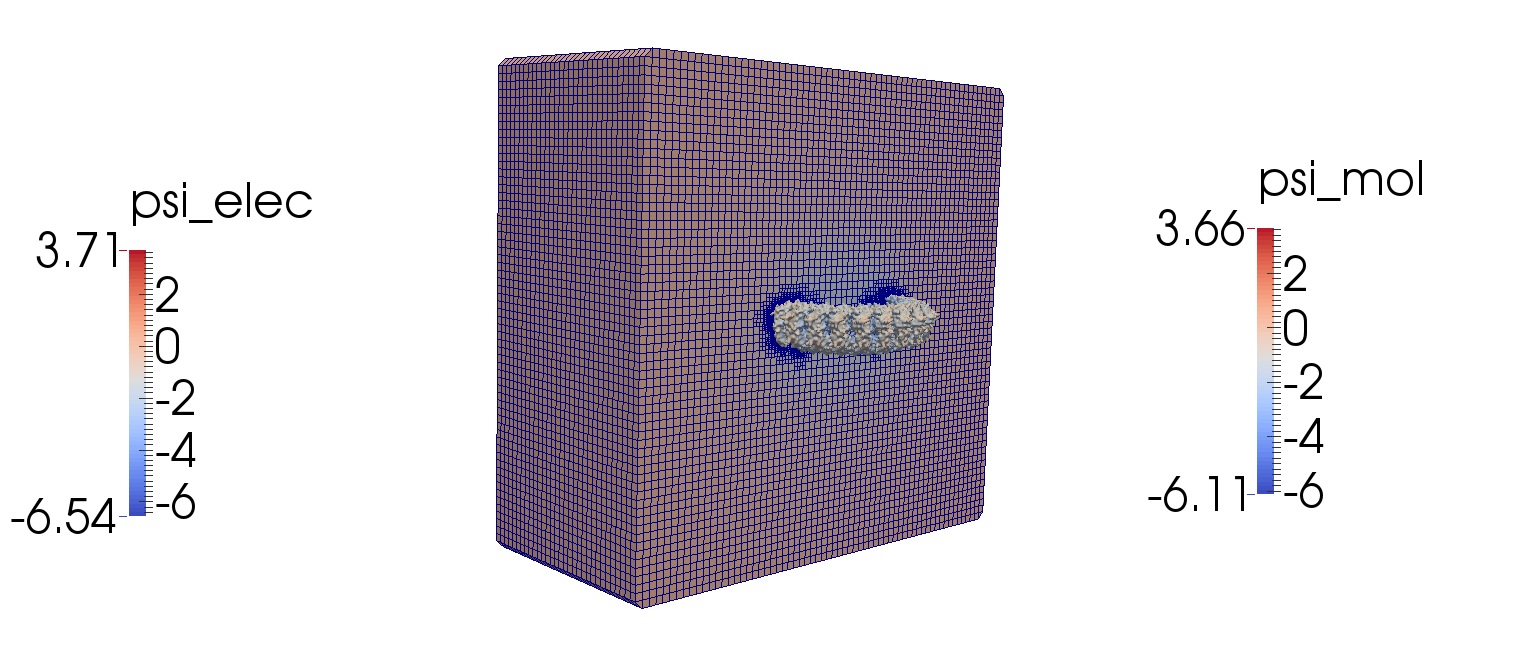
\includegraphics[width=0.945\textwidth]{../figs/3J6D_cutaway_7_10}
\end{center}
\caption{A cutaway of the computational domain (colored by bulk potential) and the computed SES surface of the 3J6D protien colored by the electric potential on its surface.} \label{fig:3J6D_cutaway_7_!0}
\end{figure}


\begin{figure}[ht]
\begin{center}
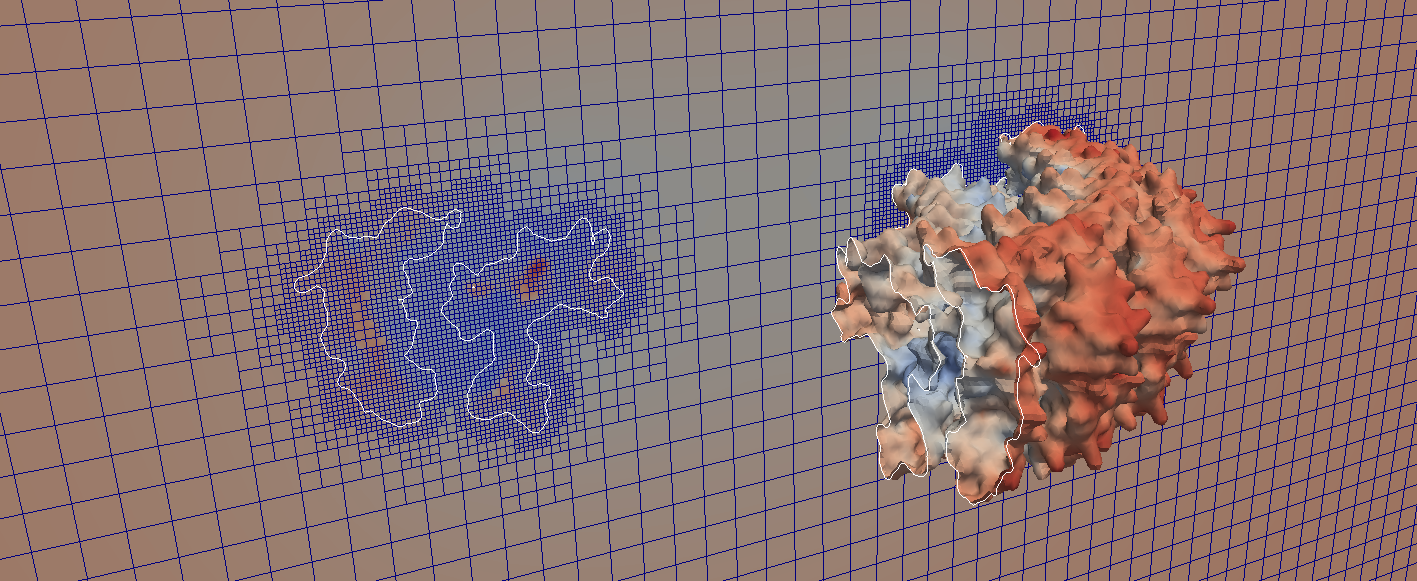
\includegraphics[width=0.945\textwidth]{../figs/3J6D_zoom_7_10}
\end{center}
\caption{Zoomed in version} \label{fig:3J6D_zoom_7_10}
\end{figure}



\section{Conclusion}\label{sec::conclusion}


\bibliography{references}


\end{document}
